\documentclass[conference]{IEEEtran}
\IEEEoverridecommandlockouts
% The preceding line is only needed to identify funding in the first footnote. If that is unneeded, please comment it out.
\usepackage{cite}
\usepackage{amsmath,amssymb,amsfonts}
\usepackage{algorithmic}
\usepackage{graphicx}
\usepackage{textcomp}
\usepackage{xcolor}
\usepackage{booktabs}
\usepackage{array}
\usepackage{url}
\usepackage{amsmath}
\usepackage{siunitx}
\def\BibTeX{{\rm B\kern-.05em{\sc i\kern-.025em b}\kern-.08em
    T\kern-.1667em\lower.7ex\hbox{E}\kern-.125emX}}
\begin{document}

\title{AudioGraph: Busca em grafo para geração se sequências de músicas \\

\thanks{}
}


\author{
\begin{tabular}{cc}
\text{José Ryan Santos de Melo} &
\text{Adley Silva Mendes} \\

\textit{jose.ryan.santos.de.melo@ccc.ufcg.edu.br} &
\textit{adley.silva.mendes@ccc.ufcg.edu.br} \\

124110896 & 124110612 \\[1em]

\text{Hugo Victor Santos Pinheiro da Silva} &
\text{Higor Albuquerque Feitoza} \\

\textit{hugo.victor.santos.pinheiro.da.silva@ccc.ufcg.edu.br} &
\textit{higor.albuquerque.feitoza@ccc.ufcg.edu.br} \\

124110914 & 123110247 \\[1em]

\text{Kayo Emanuel Salvino do Nascimento} &
\text{Iury Ruan do Nascimento Santos} \\

\textit{kayo.emanuel.salvino.do.nascimento@ccc.ufcg.edu.br} &
\textit{iury.ruan.do.nascimento.santos@ccc.ufcg.edu.br} \\

20250019080 & 124110855
\end{tabular}
}


\maketitle


\section{Introdução}

Este projeto faz a implementação de um sistema de busca em grafo para criar sequências de músicas, baseando-se em
features e semelhança entre músicas, além disso, o algoritmo possui uma semente de aleatoriedade para realizar
a recomendação de música.

\section{Dataset de músicas}

\subsection*{Spotify Tracks Dataset}

O dataset usado para esse projeto foi o Spotify Tracks Dataset \cite{b1}. Esse dataset está disponível na plataforma do Hugging Face e pode ser baixado gratuitamente. A escolha se deu por ser um dataset com inúmeras amostras, possuindo 114 mil amostras e mais de 125 gêneros musicais. Além disso, esse dataset possui várias features já extraídas das músicas, como por exemplo: dançabilidade, energia, acusticidade entre muitas outras.

\subsection*{iTunes e Deezer}

O Spotify limitou sua API descontinuando a função de retornar um link para preview da música \cite{b2}, devido a isso não foi possível obter as músicas através de requisições a API oficial e baixar mais 114 mil músicas seria inviável. Como alternativa, decidimos usar as API do Itunes e Deezer para complementar essa falta, nessas APIs a busca pela música se dá pelo autor e pelo nome da música, entretanto elas ainda possuem limitações, como por exemplo o Itunes que fornece apenas uma preview de 30 segundos da música. De todo modo, as APIs do iTunes e Deezer estão mais atualizada e fornecem mais músicas que o disponilibilazado pelo Spotify, que é um dataset de 2024.

\section{Arquitetura e implementação}

Para a arquitetura decidimos usar um grafo ponderado dirigido, em que cada vértice representa uma música e as arestas entre os vértices representam a correlação entre as duas músicas.

O projeto é dividido em: coleta dos dados, normalização dos dados, coleta de features,
construção do grafo e por fim o algoritmo de recomendação.

\begin{figure}[htbp]
    \centering
    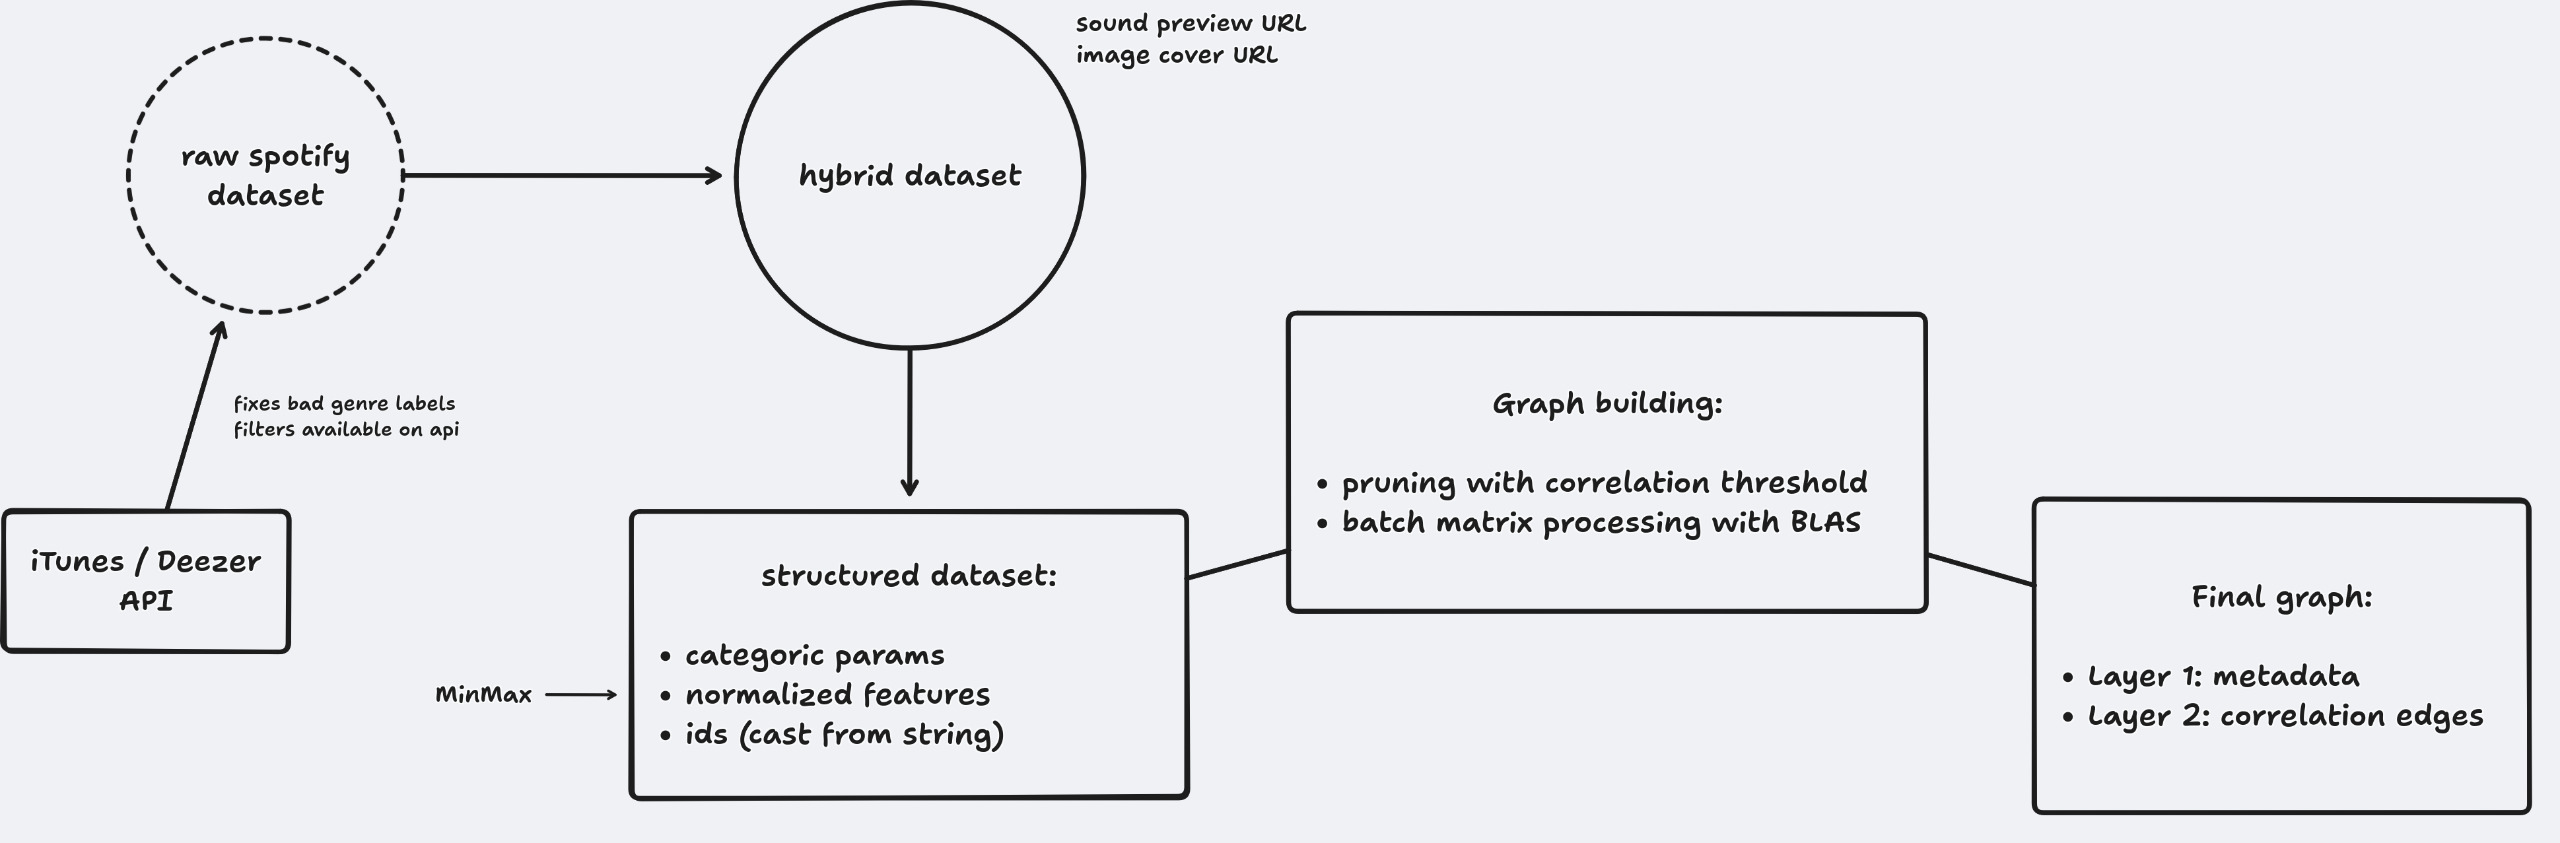
\includegraphics[width=0.4\textwidth]{images/fluxo_de_dados.jpeg}
    \caption{Fluxo de dados.}
    \label{fig:fluxo-de-dados}
\end{figure}

\begin{figure}[htbp]
    \centering
    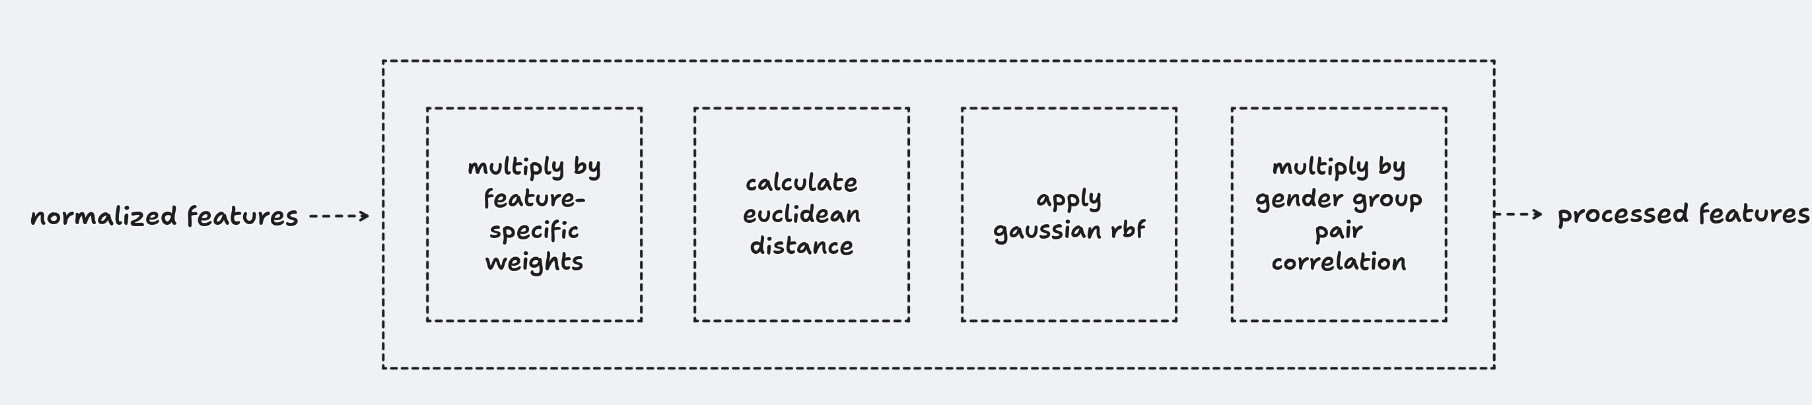
\includegraphics[width=0.4\textwidth]{images/normalizacao.jpeg}
    \caption{Normalização dos dados.}
    \label{fig:normalizacao-dos-dados}
\end{figure}

\begin{figure}[htbp]
    \centering
    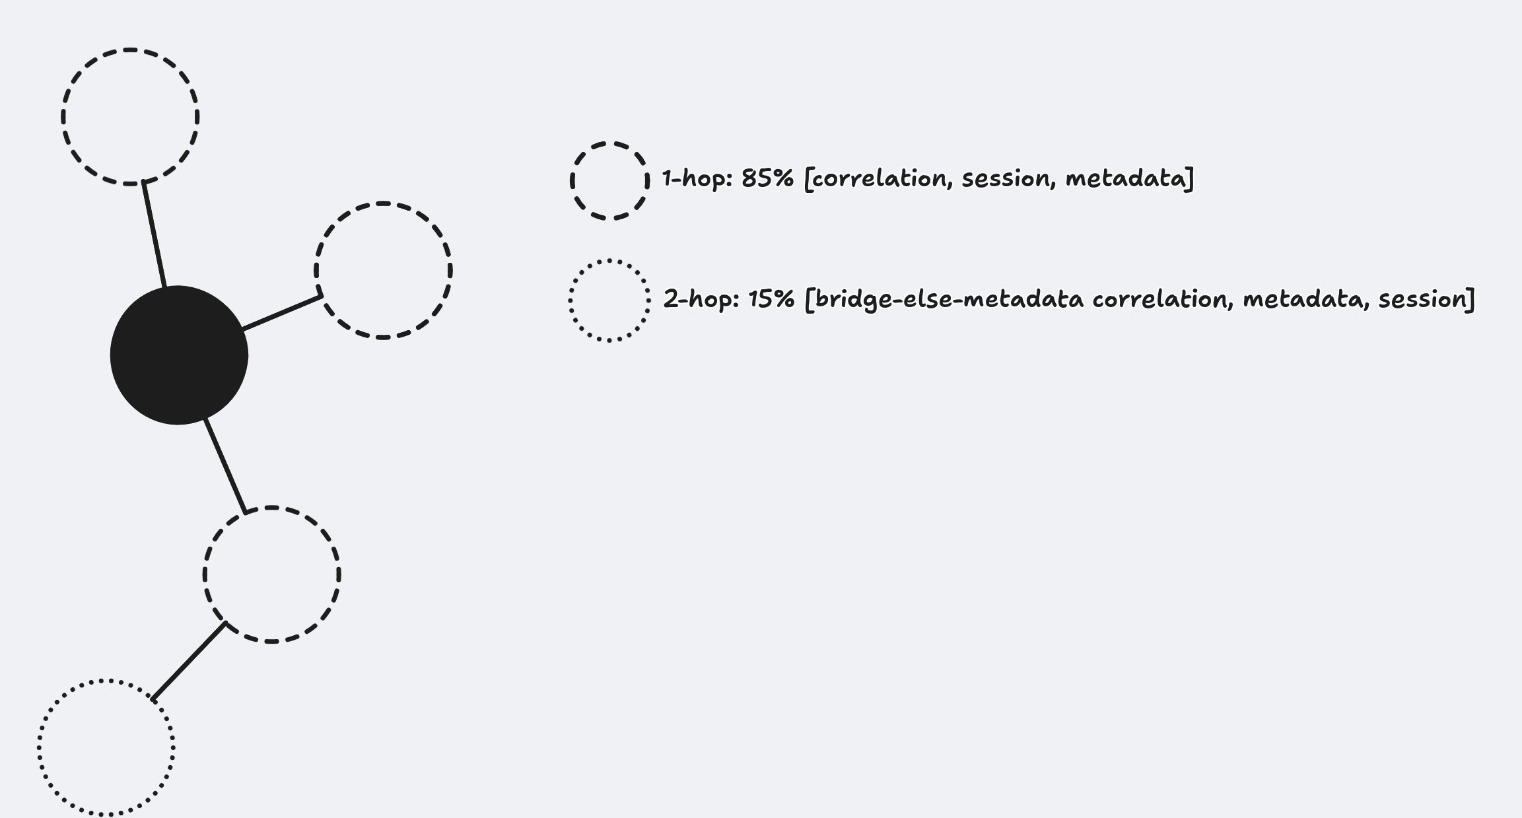
\includegraphics[width=0.3\textwidth]{images/algoritmo_recomendacao.jpeg}
    \caption{Algoritmo de recomendação.}
    \label{fig:algoritmo-de-recomendacao}
\end{figure}

\section{Criação do grafo e features}

Como foi definido, no grafo cada vértice representa a música, e cada aresta representa uma conexão de semelhança entre as músicas. Para a construção desse, cada aresta possuí um peso,
esse peso representa a semelhança entre as músicas, ou mais detalhadamente esse peso é representado pela
a equação \ref{eq:peso}. Dessa forma, um caminho com músicas muito semelhantes terá um custo
menor, sendo ele mais favorecido pelo algoritmo.

\begin{equation}
\label{eq:peso}
    peso = 1 - semelhança
\end{equation}

Para o cálculo do peso foram escolhidas features que conseguem representar bem semelhança entre músicas [3], sendo elas: danceability, energy, valence, tempo\_norm, acousticness, instrumentalness, speechiness, loudness\_norm e liveness.

Inicialmente, a criação de arestas é completa, porém ela precisa ser podada para que o grafo
caiba na memória. Essa poda é feita através de um limiar de correlação, definimos esse limiar
com o valor de 30\%. Ou seja, se a semelhança for menor ou igual a 30\%, não criamos uma
aresta a priori entre duas músicas.

Além disso, para cada nó do grafo adicionamos mais atributos, como autor, albúm etc. Esses metadados serão uteis para realizar a busca nas APIs do iTunes e Deezer como também para uma
futura melhora do algoritmo.

\section{Algoritmo de busca}

O algoritmo de busca realiza a geração da sequência a partir de dois casos e duas probabilidades. O primeiro caso consiste em buscar músicas a partir de uma distância do nó
atual e a distância de um nó desejado. Essas distâncias podem ser de 1 ou 2, com probabilidades de $85\%$ e $15\%$, respectivamente. 

O segundo caso, refere-se a buscar o nó com a maior semelhança, ou seja, o nó com o menor peso. Dessa forma, o algoritmo segue o seguinte passo: escolhe probabilisticamente qual distância irá buscar, definida a distância ele escolhe as k maiores similaridades entre a
música atual e uma potencial próxima música, feito isso ele retorna as k-músicas mais 
semelhantes entre as selecionadas. Por fim, se o usuário continuar por esse caminho o
algoritmo continua expandindo músicas semelhantes as anteriores.


\section{Problemas encontrados}

\subsection*{Músicas acusticamente próximas, vibes opostas}

Um dos problemas encontrados ao usar apenas as features como forma de realizar a criação
de semelhanças foi que em alguns casos, músicas com features muito próximas, possuiam
"vibes" ou teor diferentes. Para resolver essa falha, realizamos a separação das músicas
em "super gêneros" e separamos manualmente a correlação entre essas músicas. Como por exemplo, músicas do gênero eletrônica, garage, party são naturalmente muito semelhantes,
dado isso separamos elas em um super gênero, nesse caso seria o super gênero "Eletrônica".

Outro caso é que o dataset possuia músicas de gêneros pouco conhecidos e muito nichados, desse modo a separação permitiu diminuir a recomendação a priori para esses gêneros, mas, ao recomendar, melhorar a probabilidade de recomenda-los novamente caso o usuário goste daquela sequência.


\subsection{Algoritmo míope}

Teste

\section{Métricas}

Para obter as métricas foram realizadas 100 execuções do algoritmo em uma versão menor do dataset
com 1000 amostras. Para garantir uma boa representatividade dessa amostra foi feita uma análise exploratória dos dados usando o teste t de Welch para amostras independentes e o teste KS para comparar a distribuição, isso a um nível de confiança de $\alpha = 5\%$.

Como resultado dos testes obtivemos a tabela \ref{tab:representativeness_analysis} que mostrou que os 
dados tem uma boa representatividade. Além disso, os 
gráficos \ref{fig:distribuicao-categorica} e \ref{fig:distribuicao-numerica} que 
comparam ambos os datasets se mostraram coerentes com os resultados dos testes.


\begin{figure}[htbp]
    \centering
    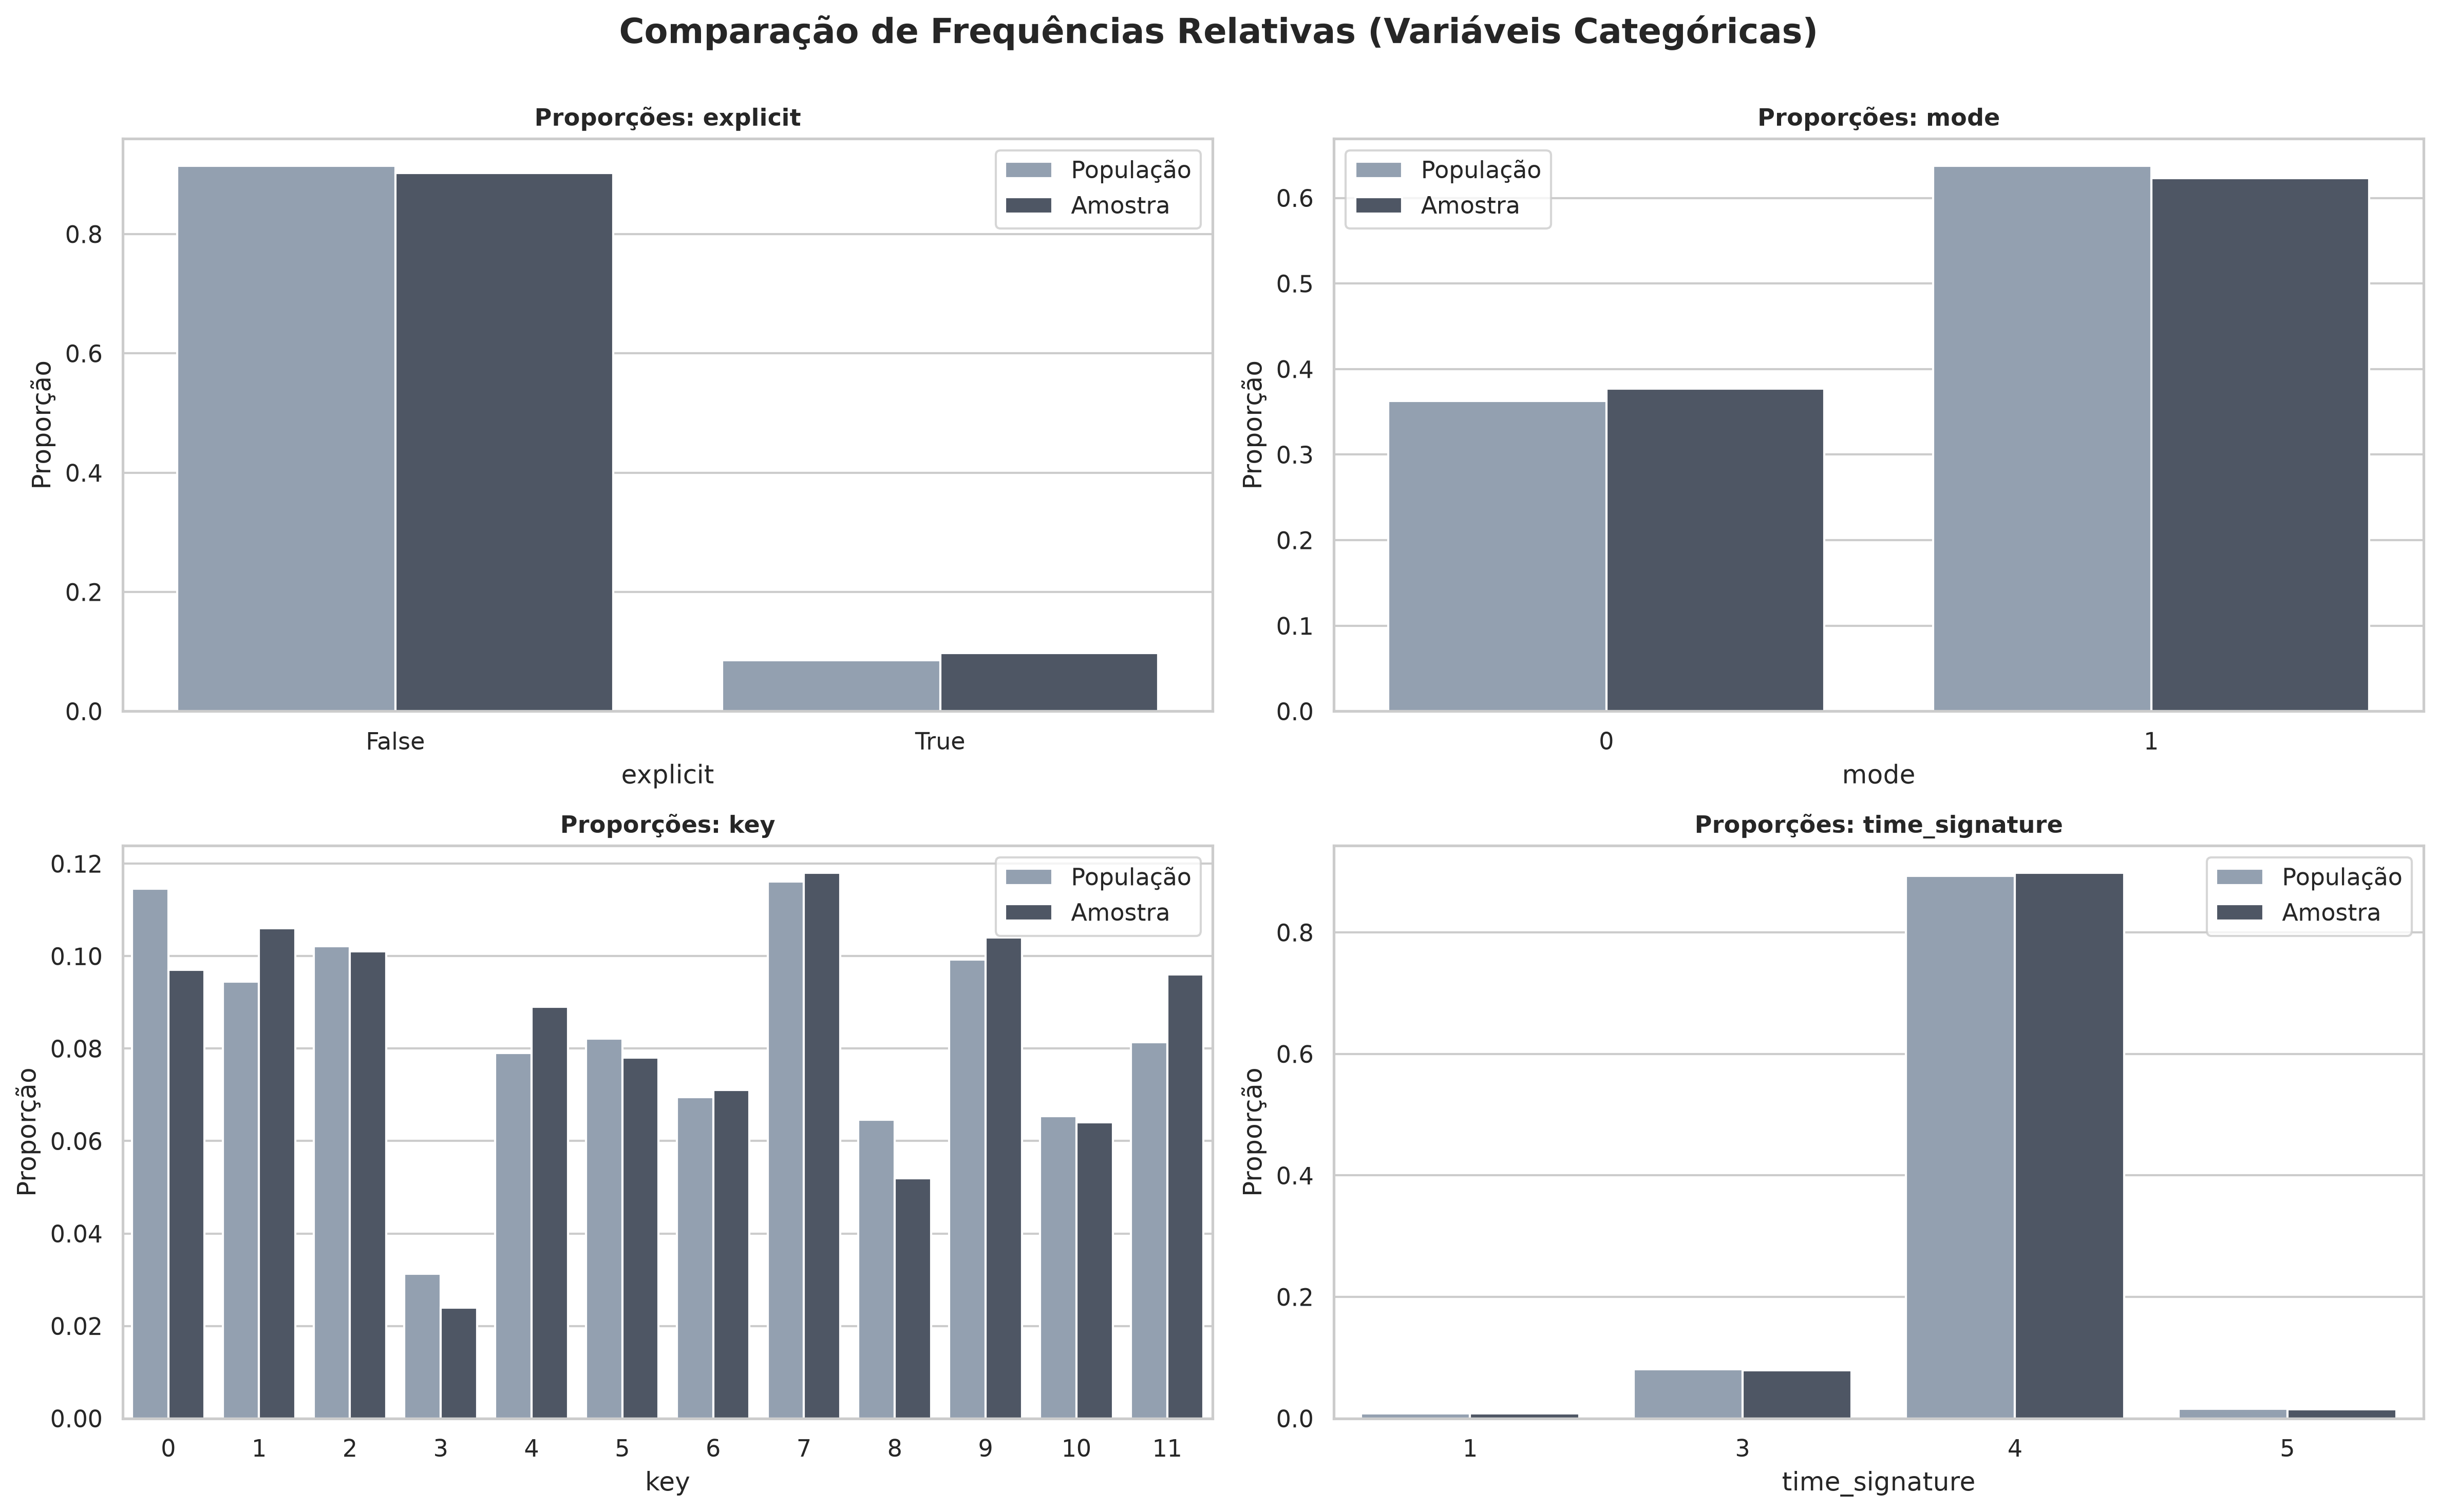
\includegraphics[width=0.4\textwidth]{images/distribuicao_categoricas.png}
    \caption{Densidade da distribuição amostral de variáveis categóricas.}
    \label{fig:distribuicao-categorica}
\end{figure}

\begin{figure}[htbp]
    \centering
    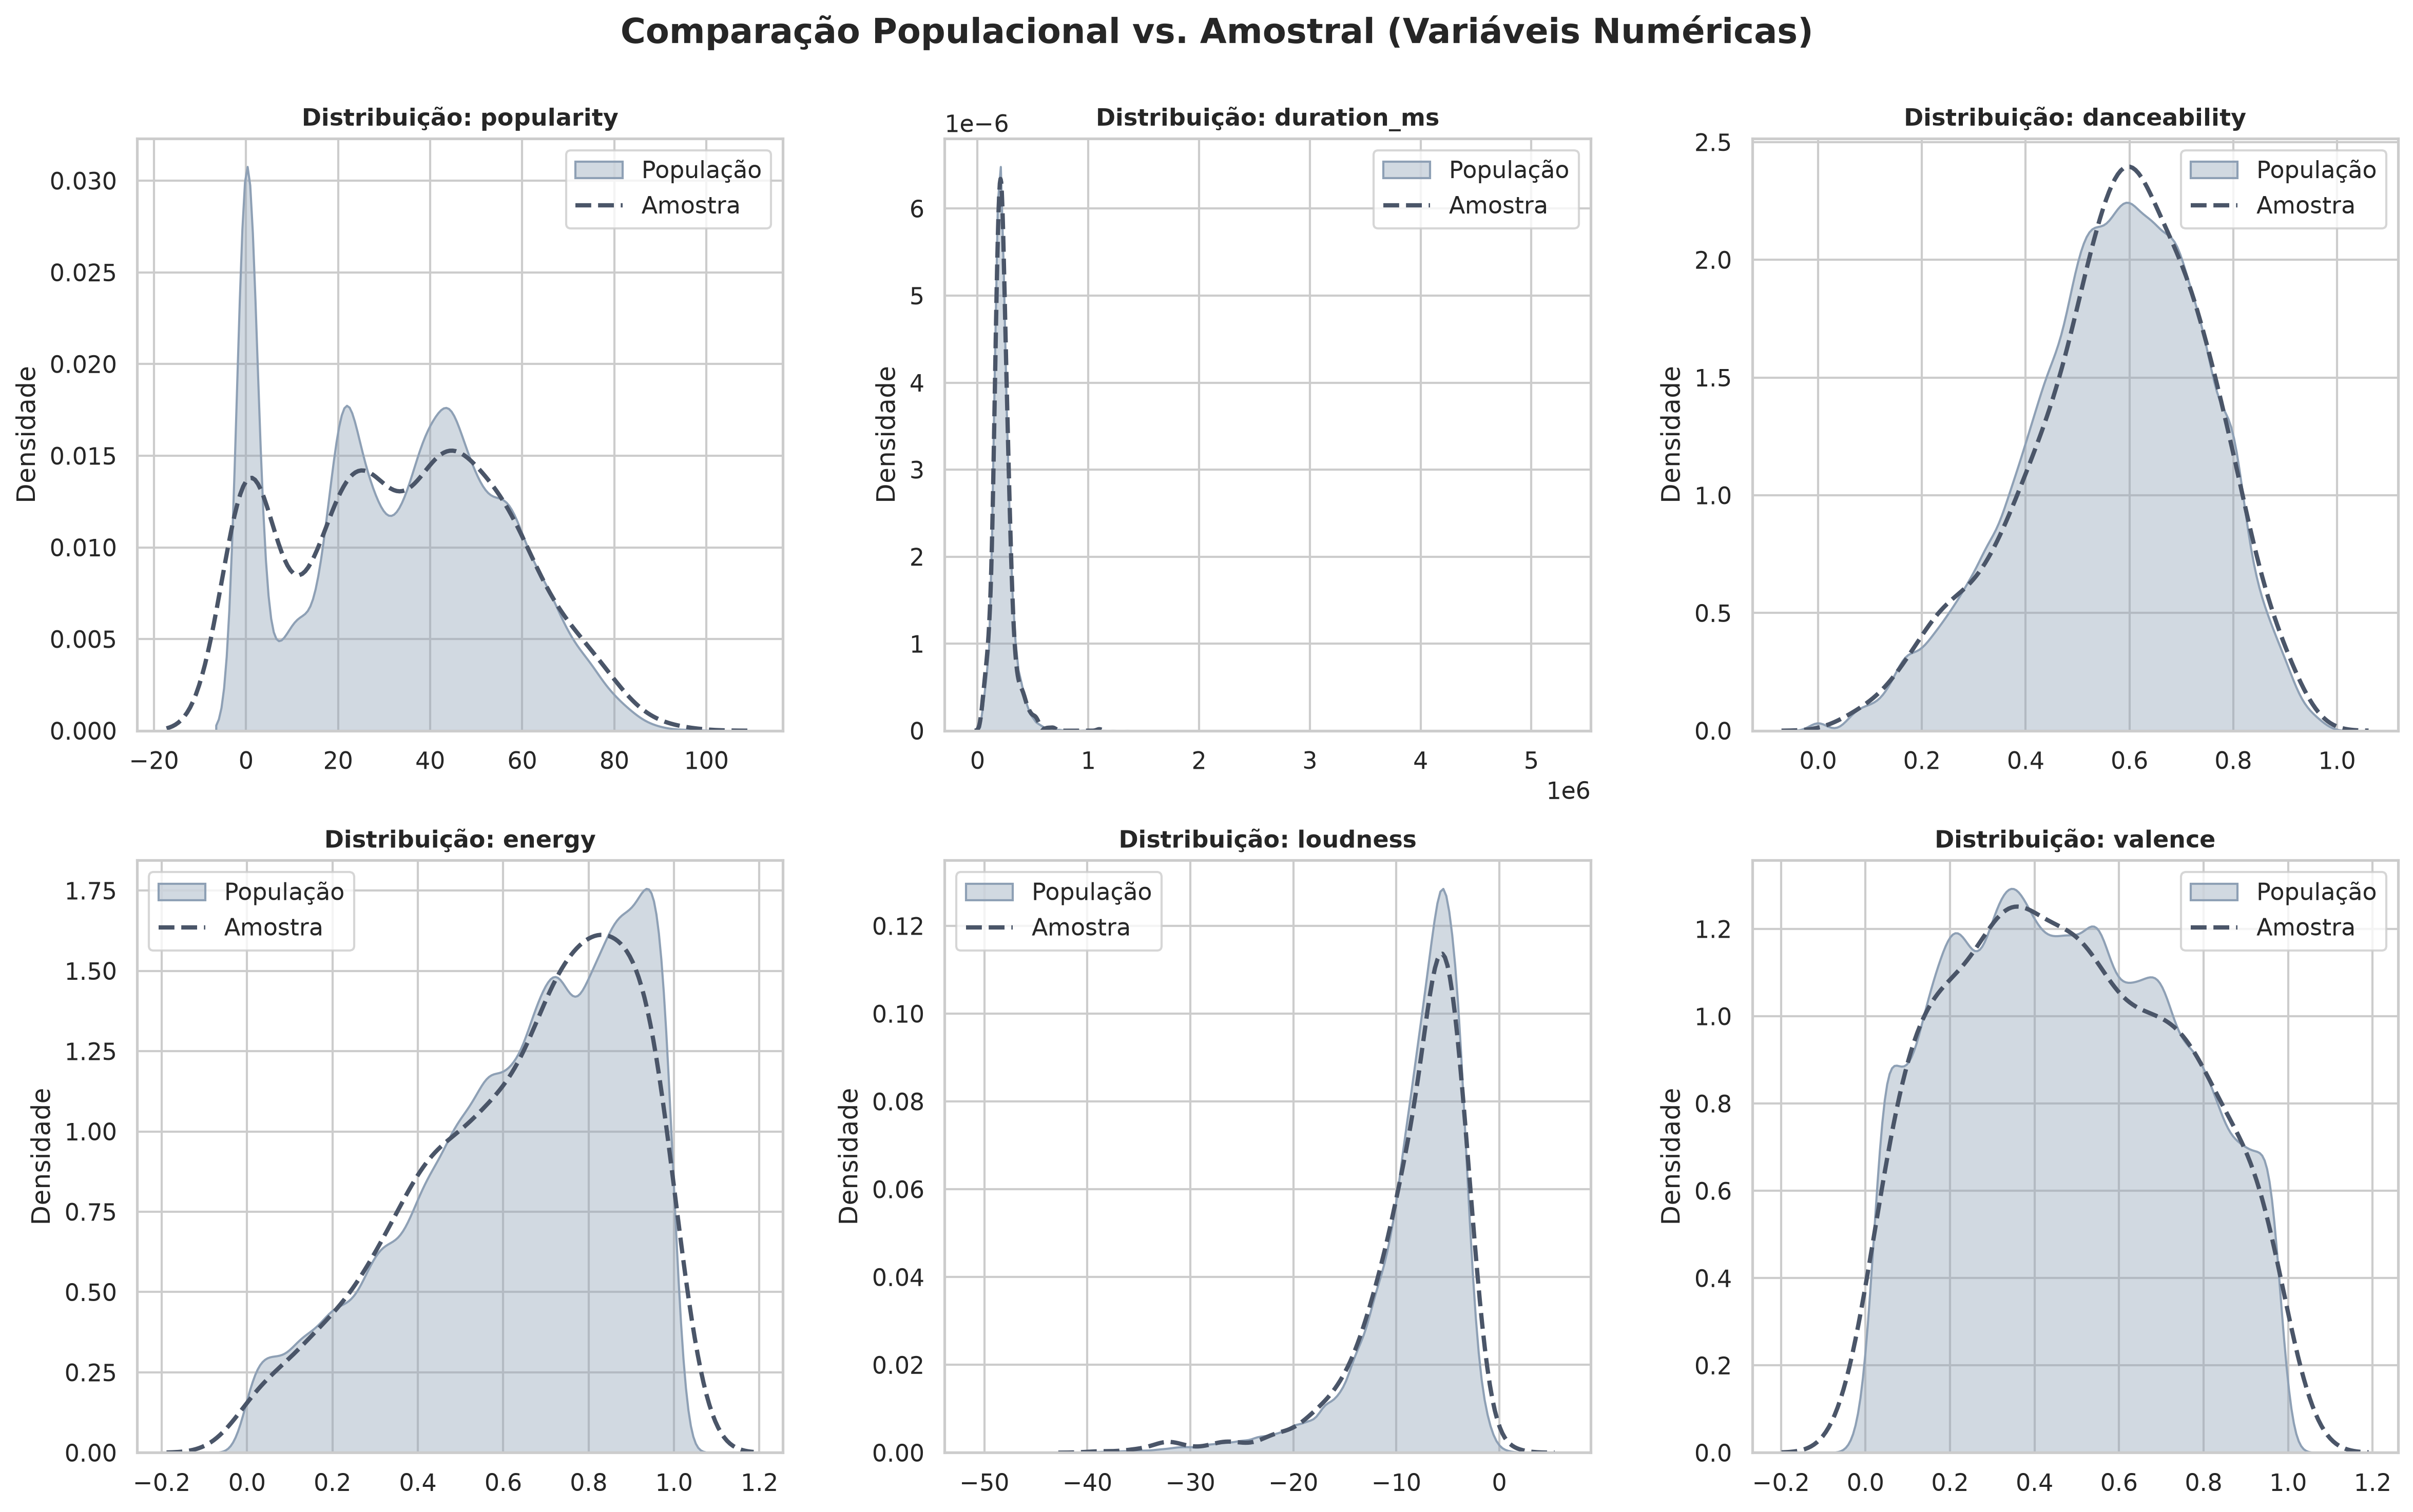
\includegraphics[width=0.3\textwidth]{images/distribuicao_numericas.png}
    \caption{Densidade da distribuição amostral de variáveis numéricas.}
    \label{fig:distribuicao-numerica}
\end{figure}


\begin{table*}[!t]
\centering
\caption{Representatividade do Dataset Small em comparação ao Dataset Full}
\label{tab:representativeness_analysis}
\begin{tabular}{l rr rr r c c c}
\toprule
\multicolumn{9}{c}{\textbf{Summary:}} Total Features = 11 \quad|\quad Statistically Representative = 11 (100.00\%) \\
\midrule
\multicolumn{9}{c}{\textbf{\scshape Variáveis numéricas (Means, SD, 95\% CI, and Sample $t$-Test)}} \\
\midrule
& \multicolumn{2}{c}{\textbf{Mean}} & \multicolumn{2}{c}{\textbf{Standard Deviation}} & \textbf{Diff.} & \textbf{Sample 95\% CI} & \textbf{$p$-value} & \textbf{Rep.?} \\
\cmidrule(lr){2-3} \cmidrule(lr){4-5}
\textbf{Feature} & \textbf{Full} & \textbf{Small} & \textbf{Full} & \textbf{Small} & \textbf{(\%)} & \textbf{[Lower, Upper]} & ($t$-test) & ($\alpha=0.05$) \\
\midrule
energy           & 0.6414     & 0.6408     & 0.2515     & 0.2501    & 0.09 & [0.625, 0.656]         & 0.9410 & Yes \\
instrumentalness & 0.1560     & 0.1562     & 0.3096     & 0.3064    & 0.10 & [0.137, 0.175]         & 0.9868 & Yes \\
tempo            & 122.1478   & 122.3406   & 29.9782    & 29.2995   & 0.16 & [120.522, 124.159]     & 0.8353 & Yes \\
duration\_ms     & 228029.15  & 227007.23  & 107297.71  & 88090.62  & 0.45 & [221540.80, 232473.67] & 0.7138 & Yes \\
valence          & 0.4741     & 0.4763     & 0.2593     & 0.2635    & 0.46 & [0.460, 0.493]         & 0.7918 & Yes \\
loudness         & -8.2590    & -8.3042    & 5.0293     & 5.3586    & 0.55 & [-8.637, -7.972]       & 0.7897 & Yes \\
danceability     & 0.5668     & 0.5721     & 0.1735     & 0.1724    & 0.93 & [0.561, 0.583]         & 0.3328 & Yes \\
popularity       & 33.2385    & 33.5760    & 22.3051    & 22.9051   & 1.02 & [32.155, 34.997]       & 0.6414 & Yes \\
acousticness     & 0.3149     & 0.3110     & 0.3325     & 0.3291    & 1.25 & [0.291, 0.331]         & 0.7056 & Yes \\
liveness         & 0.2136     & 0.2183     & 0.1904     & 0.1960    & 2.23 & [0.206, 0.230]         & 0.4429 & Yes \\
speechiness      & 0.0847     & 0.0898     & 0.1057     & 0.1167    & 6.11 & [0.083, 0.097]         & 0.1614 & Yes \\
\midrule
\multicolumn{9}{c}{\textbf{\scshape Variáveis categóricas}} \\
\midrule
\multicolumn{3}{l}{\textbf{Categorical Feature}} & \multicolumn{3}{c}{\textbf{Max Deviation (percentage points)}} & \multicolumn{3}{c}{\textbf{Mean Deviation (percentage points)}} \\
\midrule
\multicolumn{3}{l}{explicit}       & \multicolumn{3}{c}{1.25\%} & \multicolumn{3}{c}{1.25\%} \\
\multicolumn{3}{l}{key}            & \multicolumn{3}{c}{1.76\%} & \multicolumn{3}{c}{0.74\%} \\
\multicolumn{3}{l}{mode}           & \multicolumn{3}{c}{1.46\%} & \multicolumn{3}{c}{1.46\%} \\
\multicolumn{3}{l}{time\_signature} & \multicolumn{3}{c}{0.46\%} & \multicolumn{3}{c}{0.19\%} \\
\multicolumn{3}{l}{track\_genre}    & \multicolumn{3}{c}{0.08\%} & \multicolumn{3}{c}{0.04\%} \\
\bottomrule
\end{tabular}
\end{table*}



\vspace{12pt}

\newpage

\newpage

\begin{thebibliography}{00}
\bibitem{b1} Spotify Tracks Dataset. Disponível: \url{https://huggingface.co/datasets/maharshipandya/spotify-tracks-dataset}
\bibitem{b2} Spotify API Reference. Disponível: \url{https://developer.spotify.com/documentation/web-api/reference/get-track}
\bibitem{b3} Y. V. Srinivasa Murthy, e Shashidhar G. Koolagudi, ``Content-Based Music Information Retrieval (CB-MIR) and Its Applications toward the Music Industry: A Review''. Disponível: \url{https://dl.acm.org/doi/10.1145/3177849} 

\end{thebibliography}
\vspace{12pt}

\end{document}
